\section{Introduction}
%
%  Introduction
%
\begin{frame} {Introduction}
  The stack of tasks provides a control framework for real-time redundant manipulator control
  \pause
  \begin{itemize}
  \item implementation of a data-flow,
  \pause
  \item control of the graph by python scripting,
  \pause
  \item task-based hierarchical control,
  \pause
  \item portable: tested on HRP-2, Nao, Romeo.
\end{itemize}
\end{frame}

\section{Theoretical foundations}

%
%  Rigid body $\body$
%

\begin{frame} {Rigid body $\body$}
  \begin{itemize}
    \item Configuration represented by an homogeneous matrix
      $$
      M_{\body} = \left(\begin{array}{cc}
        \rotation_{\body} & \trans_{\body}\\
        0 \ 0 \ 0 & 1 
      \end{array}\right) \in SE(3)
      $$
      \pause
      $$
      \rotation_{\body} \in SO(3) \Leftrightarrow \rotation_{\body}^{T}\rotation_{\body} = I_3
      $$
      \pause
      Point $\x\in\real^3$ in local frame of $\body$ is moved to $\y\in\real^3$ in global frame:
      $$
      \left(\begin{array}{l}
        \y \\ 1
      \end{array}\right) =
      M_{\body} \left(\begin{array}{l} \x \\ 1
      \end{array}\right)
      $$
  \end{itemize}
\end{frame}

%
%  Rigid body $\body$
%

\begin{frame} {Rigid body $\body$}
  \begin{itemize}
    \item Velocity represented by $(\vel_{\body},\omega_{\body})\in \real^6$ where
      \pause
      $$
      \dot{\rotation}_{\body} = \hat{\omega}_{\body} \rotation_{\body}
      $$
      and
      $$
      \hat {\omega} = \left(\begin{array}{ccc}
        0 & -\omega_3 & \omega_2 \\
        \omega_3 & 0 & -\omega_1 \\
        -\omega_2 & \omega_1 & 0
        \end{array}\right)
      $$
      is the matrix corresponding to the cross product operator
      \pause
    \item Velocity of point P on $\body$
      $$
      \vel_p = \dot{\trans}_{\body} + \omega_{\body} \times \vec{O_{\body}P}
      $$
      where $O_{\body}$ is the origin of the local frame of $\body$.
  \end{itemize}
\end{frame}

%
%  Configuration space
%

\begin{frame} {Configuration space}
  \parbox{.71\linewidth} {
  \begin{itemize}
    \item Robot: set of rigid-bodies linked by joints $\body_0,\cdots\body_m$.
      \pause
    \item Configuration: position in space of each body.
      $$
      \begin{array}{l}
        \conf = (\conf_{waist}, \theta_1, \cdots \theta_{n-6}) \in SE(3) \times \real^{n-6}\\
        \conf_{waist} = (x, y, z, roll, pitch, yaw)
      \end{array}
      $$
  \end{itemize}
  }
  \parbox {.28\linewidth} {
    \centerline {
      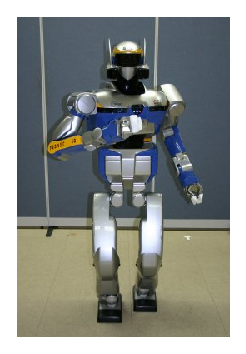
\includegraphics[width=\linewidth]{figures/hrp2}
    }
  }
  \pause
  \begin{itemize}
  \item Position of $\body_i$ depends on $\conf$:
    $$M_{\body_i} (\conf) \in SE(3)$$
    
  \end{itemize}
\end{frame}

%
%  Velocity
%

\begin{frame} {Velocity}
  \parbox{.71\linewidth} {
  \begin{itemize}
    \item Velocity: 
    \begin{eqnarray*}
      \dot{\conf} &=& (\dot{x}, \dot{y}, \dot{z}, \omega_{x}, \omega_{y}, \omega_{z},\dot{\theta}_1,\cdots \dot{\theta}_{n-6})\\
      \omega &\in& \real^3
    \end{eqnarray*}
  \pause
  \item Velocity of $\body_i$
  \end{itemize}
  }
  \parbox {.28\linewidth} {
    \centerline {
      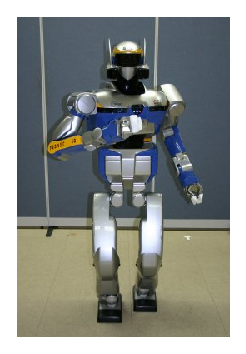
\includegraphics[width=\linewidth]{figures/hrp2}
    }
  }
  \pause
   $$
    \left(\begin{array}{l} \vel_{\body_i} \\ \omega_{\body_i}\end{array}\right) (\conf, \dot{\conf}) = J_{\body_i} (\conf).\dot{\conf} \in \real^6
    $$
\end{frame}

%
% Task
%

\begin{frame} {Task}
  \begin {itemize}
    \item Definition: function of the
      \begin {itemize}
        \item robot configuration, 
        \item time and
        \item possibly external parameters
      \end{itemize}
      that should converge to 0:
      $$
      T \in C^{\infty} (\CS\times\real, \real^m)
      $$
      \pause
      \item Example: position tracking of an end-effector $\body_{ee}$
        \pause
        \begin{itemize}
        \item $M (\conf) \in SE(3)$ position of the end-effector,
        \pause
        \item $M^{*} (t) \in SE(3)$ reference position
        \end{itemize}
        \pause
        $$
        T (\conf, t) = \left(\begin{array}{cc}
          \trans (M^{* -1}(t) M (\conf)) \\
          \utheta (R^{* -1}(t) R (\conf))
        \end{array}\right)
        $$
        where
        \begin{itemize}
          \item $\trans ()$ is the translation part of an homogeneous matrix,
          \item $R$ and $R^{*}$ are the rotation part of $M$ and $M^{*}$.
        \end{itemize}
        
  \end {itemize}
\end{frame}

%
%  Hierarchical task based control
%

\begin{frame} {Hierarchical task based control}
  Given
  \begin{itemize}
  \item a configuration $\conf$,
  \item two tasks of decreasing priorities:
    \begin{itemize}
      \item $T_1 \in C^{\infty}(\CS\times\real, \real^{m_1})$,
      \item $T_2 \in C^{\infty}(\CS\times\real, \real^{m_2})$,
    \end{itemize}
  \end{itemize}
  \pause
  compute a control vector $\dot{\conf}$
  \begin{itemize}
    \item that makes $T_1$ converge toward 0 and
    \item that makes $T_2$ converge toward 0 if possible.
  \end{itemize}
\end{frame}

%
%  Hierarchical task based control
%

\begin{frame} {Hierarchical task based control}
  Jacobian:
  \begin{itemize}
  \item we denote
    \begin{itemize}
      \item $J_i = \frac{\partial T_i}{\partial \conf}$ for $i\in\{1,2\}$
  \end{itemize}
    \pause
  \item then
    \begin{itemize}
    \item $\forall\conf\in\CS,\forall t\in\real, \forall\dot{\conf}\in\real^n,\ \dot{T}_i = J_i(\conf, t) \dot{\conf} + \frac{\partial T_i}{\partial t} (\conf, t)$
    \end{itemize}
  \end{itemize}
  \pause
  We try to enforce
  \begin{itemize}
    \item $\dot{T}_1 = - \lambda_1 T_1\ \ \ \Rightarrow\ \ \ T_1(t) = e^{-\lambda_1 t}T_1(0)\rightarrow 0$
      \pause
    \item $\dot{T}_2 = - \lambda_2 T_2\ \ \ \Rightarrow\ \ \ T_2(t) = e^{-\lambda_2 t}T_2(0)\rightarrow 0$
      \pause
    \item $\lambda_1$ and $\lambda_2$ are called the gains associated to $T_1$ and $T_2$.
  \end{itemize}
\end{frame}

%
%  Moore Penrose pseudo-inverse
%

\begin{frame} {Moore Penrose pseudo-inverse}
  Given a matrix $A\in\real^{m\times n}$, the Moore Penrose pseudo inverse $A^+\in\real^{n\times m}$ of $A$ is the unique matrix satisfying:
  \begin{eqnarray*}
    A A^{+} A &=& A \\
    A^{+} A A^{+} &=& A^{+} \\
    (AA^{+})^T &=& AA^{+} \\
    (A^{+}A)^T &=& A^{+}A \\
  \end{eqnarray*}
  \pause
  Given a linear system:
  $$A x = b,\ \ \ \ A\in\real^{m\times n},\ x\in\real^n,\ \ b\in\real^m $$
  $x=A^{+}b$ minimizes
  \pause
  \begin{itemize}
  \item $\|Ax-b\|$ over $\real^n$,
    \pause
  \item $\|x\|$ over $\mbox{argmin}\|Ax-b\|$.
  \end{itemize}
\end{frame}

%
%  Hierarchical task based control (2)
%

\begin{frame} {Hierarchical task based control}

  Resolution of the first constraint:
  \begin{eqnarray}\label{eq:constraint-1}
    \dot{T}_1 = J_1\dot{\conf} &+& \frac{\partial T_1}{\partial t}  = - \lambda_1 T_1\\
    J_1{\color{red} \dot{\conf}} &=& - \lambda_1 T_1 - \frac{\partial T_1}{\partial t} \\
    \dot{\conf}_1 &\triangleq& -J_1 ^{+} (\lambda_1 T_1 + \frac{\partial T_1}{\partial t} )
  \end{eqnarray}
  \pause
  Where $J_1^+$ is the (Moore Penrose) pseudo-inverse of $J_1$.\\
  \pause
  $\dot{\conf}_1$ minimizes
  \begin{itemize}
  \item $\|J_1\dot{\conf} + \lambda_1 T_1 + \frac{\partial T_1}{\partial t} \| = \|\dot{T}_1 + \lambda_1 T_1\|$
    \pause
  \item $\|\dot{\conf}\|$ over \mbox{argmin} $\|J_1\dot{\conf} + \lambda_1 T_1 + \frac{\partial T_1}{\partial t} \|$
  \end{itemize}
  \pause
  Hence,
  \begin{itemize}
  \item if $\lambda_1 T_1 + \frac{\partial T_1}{\partial t} $ is in $Im(J_1)$, (\ref{eq:constraint-1}) is satisfied
  \end{itemize}

\end{frame}

%
%  Hierarchical task based control (3)
%

\begin{frame} {Hierarchical task based control}

  In fact
  $$\forall u\in\real^n,\ \ J_1 \left(\dot{\conf}_1 {\color{red} + (I_n - J_1^+J_1)u}\right) = J_1 \dot{\conf}_1$$
  \pause
    therefore,
    $$
    \dot{\conf} = \dot{\conf}_1 + (I_n - J_1^+J_1)u 
    $$
    also minimizes $\|J_1\dot{\conf} + \lambda_1 T_1 + \frac{\partial T_1}{\partial t}\|$.\\
    \vskip .8cm
    \pause
    $P_1 = (I_n - J_1^+J_1)$ is a projector on $J_1$ kernel:\\
    $J_1P_1 = 0$\\
    \pause
    $\forall u\in\real^n$, if $\dot{\conf} = P_1 u$, then, $\dot{T_1}=\frac{\partial T_1}{\partial t}$.
\end{frame}

%
%  Controlling the second task
%

\begin{frame} {Controlling the second task}
  We have
  \begin{eqnarray*}
    \dot{\conf} &=& \dot{\conf}_1 + P_1 u\\
    \dot{T}_2 &=& J_2\dot{\conf} + \frac{\partial T_2}{\partial \conf}\\
    \dot{T}_2 &=& J_2 \dot{\conf}_1 + \frac{\partial T_2}{\partial \conf} + J_2 P_1 {\color{red}u}
  \end{eqnarray*}
  \pause
  We want
  \begin{eqnarray*}
    \dot{T}_2 &=&  - \lambda_2 T_2
  \end{eqnarray*}
  \pause
  Thus
  \begin{eqnarray*}
    - \lambda_2 T_2 &=& J_2 \dot{\conf}_1 + \frac{\partial T_2}{\partial \conf} + J_2 P_1 {\color{red}u} \\
    J_2 P_1 {\color{red}u} &=& - \lambda_2 T_2 - J_2 \dot{\conf}_1 - \frac{\partial T_2}{\partial \conf}
  \end{eqnarray*}
\end{frame}

%
%  Controlling the second task
%

\begin{frame} {Controlling the second task}
  Thus
  \begin{eqnarray*}
    - \lambda_2 T_2 &=& J_2 \dot{\conf}_1 + \frac{\partial T_2}{\partial \conf} + J_2 P_1 {\color{red}u} \\
    J_2 P_1 {\color{red}u} &=& - \lambda_2 T_2 - J_2 \dot{\conf}_1 - \frac{\partial T_2}{\partial \conf}\\
  \end{eqnarray*}
  \pause
  \begin{eqnarray*}
    u &=& -(J_2P_1)^+(\lambda_2 T_2 + J_2 \dot{\conf}_1 + \frac{\partial T_2}{\partial \conf})\\
    \dot  {\conf}_2 &\triangleq& \dot{\conf}_1 + P_1 u\\
&=& \dot{\conf}_1 - P_1(J_2P_1)^+(\lambda_2 T_2 + J_2 \dot{\conf}_1 + \frac{\partial T_2}{\partial \conf})) \\
  \end{eqnarray*}
  minimizes $\|\dot{T}_2 + \lambda_2 T_2\|$ over $\dot{\conf}_1 + Ker\ J_1$.
\end{frame}

%
%  Example
%

\begin{frame} {Example}
\parbox {.49\linewidth} {
  %\movie{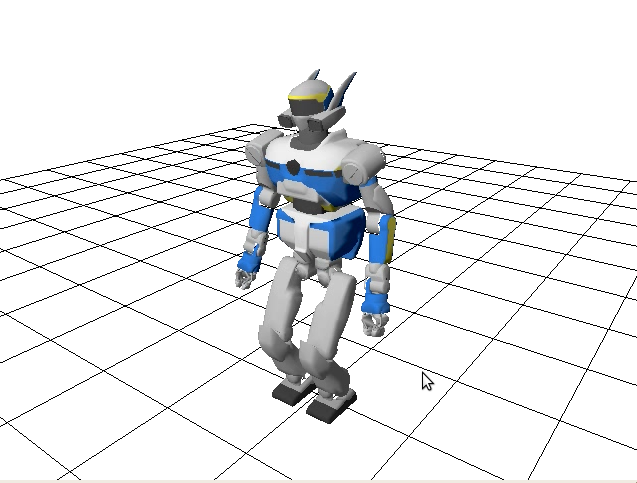
\includegraphics[width=\linewidth]{figures/sot.png}}{video/01-sot.mp4}
  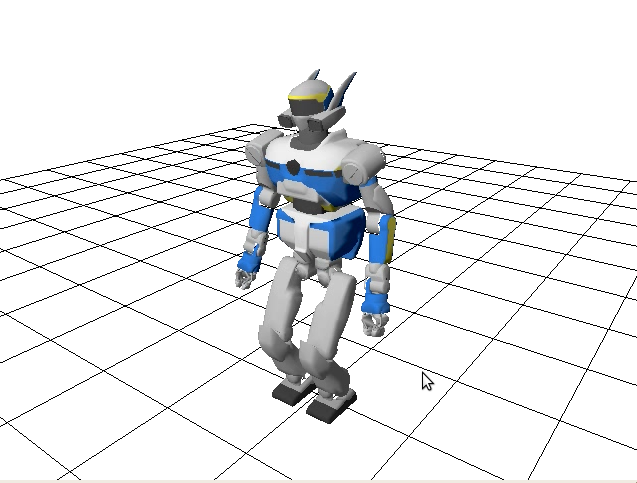
\includegraphics[width=\linewidth]{figures/sot}
}
\parbox {.5\linewidth} {
  \begin{itemize}
  \item $T_1$: position of the feet + projection of center of mass,
  \item $T_2$: position of the right wrist.
  \end{itemize}
}
\end {frame}

\section {Software}

\begin{frame} {Architecture overview}
\centerline {
  \includegraphics [height=6cm] {figures/sot-architecture}
}
\end{frame}

%
%  Libraries
%

\begin {frame} {Libraries}
  \begin{itemize}
  \item \texttt {jrl-mathtools}: implementation of small size matrices,
    \begin{itemize}
    \item to be replaced by Eigen
    \end{itemize}
    \pause
  \item \texttt {jrl-mal}: abstract layer for matrices,
    \begin{itemize}
    \item to be replaced by Eigen
    \end{itemize}
    \pause
  \item \texttt {abstract-robot-dynamics}: abstraction for humanoid robot description,
    \pause
  \item \texttt {jrl-dynamics}: implementation of the above abstract interfaces,
    \pause
  \item \texttt {jrl-walkgen}: ZMP based dynamic walk generation.
\end{itemize}
\end{frame}

%
%  dynamic-graph
%
\begin {frame} {\texttt{dynamic-graph}}
  \begin {itemize}
  \item Entity
    \begin{itemize}
    \item Signal: synchronous interface
    \item Command: asynchronous interface
    \end{itemize}
    \pause
  \item Factory
    \begin{itemize}
    \item builds a new entity of requested type,
    \item new entity types can be dynamically added (advanced).
    \end{itemize}
    \pause
  \item Pool
    \begin{itemize}
      \item stores all instances of entities,
      \item return reference to entity of given name.
    \end{itemize}
  \end{itemize}
\end {frame}

%
%  Signal
%
\begin {frame} {Signal}
  Synchronous interface storing a given data type
  \begin{itemize}
  \item output signals:
    \begin{itemize}
    \item recomputed by a callback function, or
    \item set to constant value
    \pause
    \item \textbf{warning}: setting to constant value deactivate callback,
    \end{itemize}
    \pause
  \item input signals:
    \begin{itemize}
    \item plugged by an output signal, or
    \item set to constant value,
    \pause
    \item \textbf{warning}: setting to constant value unplugs,
    \end{itemize}
  \end{itemize}
\end {frame}

%
%  Signal
%
\begin {frame} {Signal}
  Synchronous interface storing a given data type
  \begin{itemize}
  \item dependency relation: \texttt{s1} depends on \texttt{s2} if \texttt{s1} callback needs the value of \texttt{s2},
    \pause
  \item each signal \texttt{s} stores time of last recomputation in member \texttt{s.t\_}
    \pause
  \item \texttt{s} is said outdated at time \texttt{t} if
    \begin{itemize}
    \item \texttt{t > s.t\_}, and
      \pause
    \item one dependency \texttt{s\_dep} of \texttt{s}
      \begin{itemize}
      \item is out-dated or
      \item has been recomputed later than \texttt{s}: \texttt{s\_dep.t\_ > s.t\_}.
      \end{itemize}
    \end{itemize}
    \pause
  \item reading an out-dated signal triggers recomputation.
    \pause
  \item New types can be dynamically added  (advanced)
  \end{itemize}
\end {frame}

%
%  Command
%
\begin{frame} {Command}
  Asynchronous interface
  \begin{itemize}
  \item input in a fixed set of types,
  \item trigger an action,
  \item returns a result in the same set of types.
  \end{itemize}
\end{frame}

%
%  dynamic-graph-python
%
\begin {frame} {\texttt{dynamic-graph-python}}
  Python bindings to \texttt{dynamic-graph}
  \pause
  \begin{itemize}
  \item module \texttt{dynamic\_graph} linked to \texttt{libdynamic-graph.so}
  \pause
    \begin{itemize}
    \item class Entity
      \begin{itemize}
      \item each C++ entity class declared in the factory generates a python class of the same name,
      \item signals are instance members,
      \item commands are bound to instance methods
      \item method \texttt{help} lists commands
      \item method \texttt{displaySignals} displays signals
      \end{itemize}
  \pause
    \item class Signal
      \begin{itemize}
        \item property \texttt{value} to set and get signal value
      \end{itemize}
    \end{itemize}
  \pause
    \item remote interpreter to be embedded into a robot controller (advanced)
  \end{itemize}
\end{frame}

%
%  dynamic-graph-tutorial
%
\begin {frame} {\texttt{dynamic-graph-tutorial}}
  Simple use case for illustration
  \begin{itemize}
  \item Definition of 2 entity types
    \begin{itemize}
    \item \texttt{InvertedPendulum}
      \begin{itemize}
      \item input signal: \texttt{force}
      \item output signal: \texttt{state}
      \end{itemize}
    \item \texttt{FeedbackController}
      \begin{itemize}
      \item input signal: \texttt{state}
      \item output signal: \texttt{force}
      \end{itemize}
    \end{itemize}
  \end{itemize}
\end{frame}

%
%  dynamic-graph-tutorial
%
\begin {frame} {\texttt{dynamic-graph-tutorial}}
  \texttt {\tiny {>>> from dynamic\_graph.tutorial import InvertedPendulum, FeedbackController\\
      >>> \pause a = InvertedPendulum ('IP')\\
      >>> b = FeedbackController ('K')\\      
      >>> \pause a.displaySignals ()\\
      --- <IP> signal list: \\
      |-- <Sig:InvertedPendulum(IP)::input(double)::force (Type Cst) AUTOPLUGGED\\
      `-- <Sig:InvertedPendulum(IP)::output(vector)::state (Type Cst)\\
      >>> \pause a.help ()\\
      Classical inverted pendulum dynamic model\\
      \vskip .25cm
      List of commands:\\
      -----------------\\
      \begin{tabular}{ll}
      getCartMass:& Get cart mass\\
      getPendulumLength:& Get pendulum length\\
      getPendulumMass:& Get pendulum mass\\
      incr:& Integrate dynamics for time step provided as input\\
      setCartMass:& Set cart mass\\
      setPendulumLength:& Set pendulum length\\
      setPendulumMass:& Set pendulum mass\\
      \end{tabular}\\
      >>> \pause a.help ('incr')\\
      incr:\\
      \vskip .25cm
      \hspace{.5cm}Integrate dynamics for time step provided as input\\
      \vskip .25cm
      \hspace{.75cm}take one floating point number as input\\
      >>>
    }}
\end{frame}

%
%  dynamic-graph-tutorial
%
\begin {frame} {\texttt{dynamic-graph-tutorial}}
  Package provides
  \begin{itemize}
  \item C++ code of classes \texttt{InvertedPendulum} and \texttt{FeedbackController},
    \pause
  \item explanation about how to create a new entity type in C++,
    \pause
  \item information about how to create a command in C++,
    \pause
  \item information about how to create a python module defining the bindings in cmake,
    \pause
  \item python script that runs an example.
  \end{itemize}
\end{frame}

%
%  sot-core
%
\begin {frame} {\texttt{sot-core}}
Class \texttt {FeatureAbstract}
\begin{itemize}
\item function of the robot and environment states
  \pause
\begin{itemize}
  \item position of an end-effector,
  \item position of a feature in an image (visual servoing)
\end{itemize}
  \pause
\item with values in a Lie group $G$ ($SO(3)$, $SE(3)$, $\real^n$,...),
  \pause
\item with a mapping $e$ from $G$ into $\real^m$ such that
  $$ e (0_G) = 0$$
\end{itemize}
\end{frame}

%
%  Feature
%
\begin{frame} {Feature}
  When paired with a reference, features become \textit{tasks}.
  \begin{itemize}
    \item Example
      \centerline {
        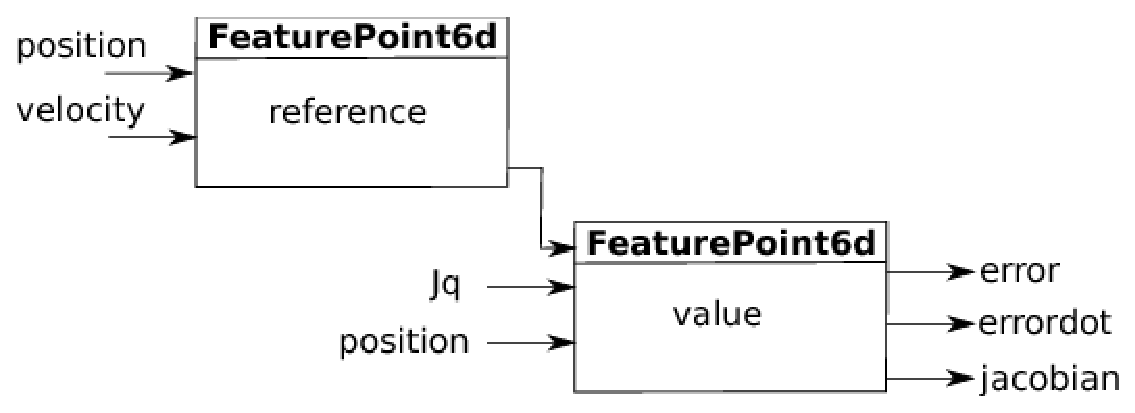
\includegraphics [width=\linewidth]{figures/feature}
      }
      \pause
    \item $\texttt {error} = e\ (\texttt {value.position} \ominus \texttt {reference.position})$
      \pause
    \item \texttt{errordot}: derivative of \texttt {error} when \texttt{value.position} is constant.
  \end{itemize}
\end{frame}

%
%  Task
% 
\begin{frame} {\texttt {Task}}
\begin {itemize}
  \item Collection of features with a control gain,
  \item implements abstraction {\color{red}\texttt{TaskAbstract}}
    \vskip .5cm
    \centerline {
      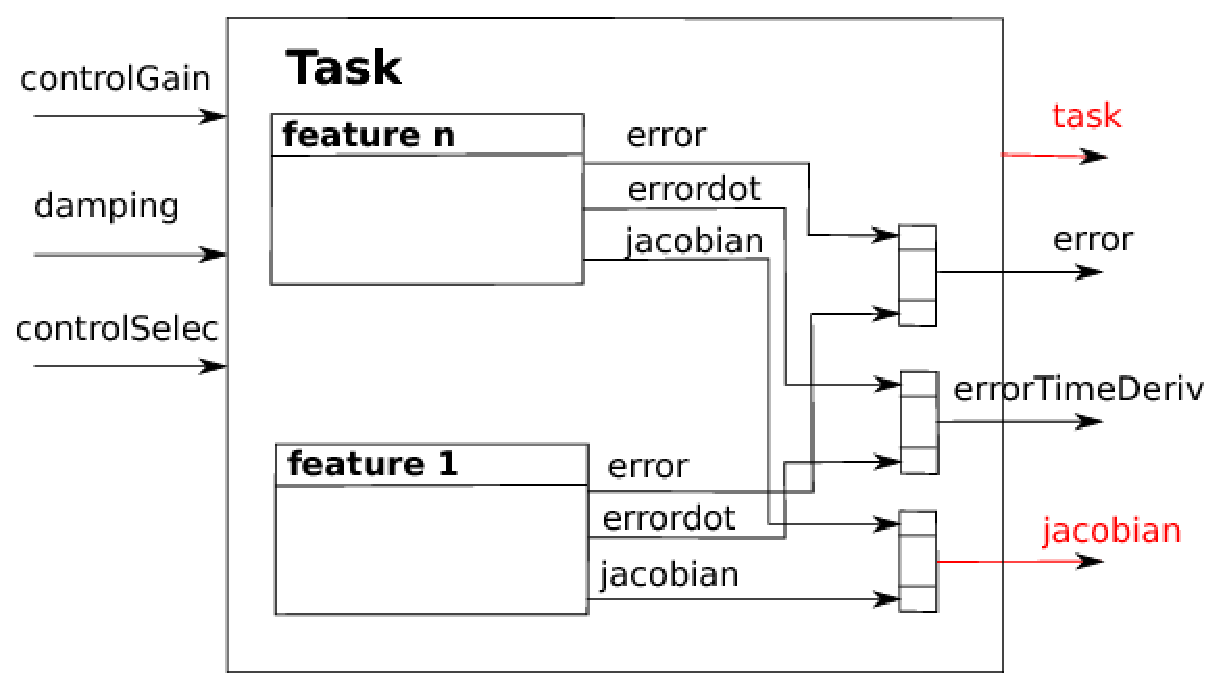
\includegraphics [width=.6\linewidth] {figures/task}
    }
  \item $\texttt{task} = - \texttt{controlGain}.\texttt{error}$
\end{itemize}
\end{frame}

%
%  Solver
%

\begin{frame} {Solver \texttt{SOT}}
  Hierarchical task solver
  \vskip .5cm
  \centerline {
    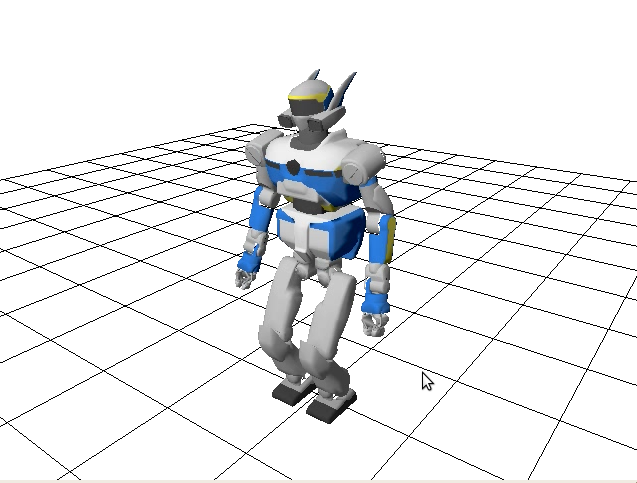
\includegraphics [width=.6\linewidth]{figures/sot}
  }
  \begin{itemize}
  \item computes robot joint velocity
  \end {itemize}
\end{frame}

%
%  \texttt {sot-dynamic}
%

\begin{frame} {\texttt{sot-dynamic}}
  \texttt{dynamic\_graph.sot.dynamics.Dynamic} builds a kinematic chain from a file and
  \begin{itemize}
  \item computes forward kinematics
    \begin{itemize}
      \item position and Jacobian of end effectors (wrists, ankles),
      \item position of center of mass
    \end{itemize}
    \item computes dynamics
    \begin{itemize}
      \item inertia matrix.
    \end{itemize}
  \end{itemize}
\end{frame}

%
%  \texttt {sot-pattern-generator}
%

\begin{frame} {\texttt{sot-pattern-generator}}
  \texttt{dynamic\_graph.sot.pattern\_generator} 
  \begin{itemize}
  \item Entity \texttt{PatternGenerator} produces walk motions as
    \begin{itemize}
      \item position and velocity of the feet
      \item position and velocity of the center of mass
    \end{itemize}
  \end{itemize}
\end{frame}

%
%  \texttt {sot-pattern-generator}
%

\begin{frame} {\texttt{sot-application}}
  \texttt{dynamic\_graph.sot.application} 
  \begin{itemize}
  \item Provide scripts for standard control graph initialization
    \begin{itemize}
      \item depends on application: control mode (velocity, acceleration)
    \end{itemize}
  \end{itemize}
\end{frame}

%
%  Packages specific to robots
%
\begin{frame} {Packages specific to robots}
  \texttt{sot-hrp2}
  \begin{itemize}
  \item defines a class \texttt{Robot} that provides
    \begin{itemize}
      \item ready to use features for feet, hands, gaze and center of mass,
      \item ready to use tasks for the same end effectors,
      \item an entity \texttt{Dynamic},
      \item an entity \texttt{Device} (interface with the robot control system)
    \end{itemize}
  \end{itemize}
  \texttt {sot-hrprtc-hrp2}
  \begin{itemize}
  \item provide an RTC component to integrate sot-hrp2 into the robot controller.
  \end{itemize}
\end{frame}

%
%  Utilities
%
\begin {frame} {Utilities}
  \begin{itemize}
  \item \texttt{dynamic\_graph.writeGraph (filename)}: writes the current graph in a file using graphviz dot format.
    \pause
  \item \texttt {dynamic\_graph.sot.core.FeaturePosition} wraps two \texttt{FeaturePoint6d}: a value and a reference,
    \pause
  \item \texttt{MetaTask6d}:
    \pause
  \item \texttt{MetaTaskPosture}:
    \pause
  \item \texttt{MetaTaskKine6d}:
    \pause
  \item \texttt{MetaTaskKinePosture}:
    \pause
  \item \texttt{MetaTaskCom}:
  \end{itemize}
\end{frame}

%
%  Installation
%

\begin{frame} {Installation}
  Through \texttt {robotpkg}
  \begin{itemize}
  \item \texttt {\tiny git clone http://trac.laas.fr/git/robots/robotpkg.git\\
    cd robotpkg\\
    ./bootstrap/bootstrap --prefix=<your\_prefix>\\
    cd motion/sot-dynamic\\
    make install}
  \end{itemize}
\end{frame}

\begin{frame} {Installation}
  Through github:
  \begin{itemize}
  \item \texttt {\tiny
    git clone --recursive git://github.com/jrl-umi3218/jrl-mal.git\\
    git clone --recursive git://github.com/jrl-umi3218/jrl-mathtools.git\\
    git clone --recursive git://github.com/laas/abstract-robot-dynamics.git\\
    git clone --recursive git://github.com/jrl-umi3218/jrl-dynamics.git\\
    git clone --recursive git://github.com/jrl-umi3218/jrl-walkgen.git\\
    git clone --recursive git://github.com/jrl-umi3218/dynamic-graph.git\\
    git clone --recursive git://github.com/jrl-umi3218/dynamic-graph-python.git\\
    git clone --recursive git://github.com/jrl-umi3218/sot-core.git\\
    git clone --recursive git://github.com/laas/sot-tools.git\\
    git clone --recursive git://github.com/jrl-umi3218/sot-dynamic.git\\
    git clone --recursive git://github.com/jrl-umi3218/sot-pattern-generator.git\\
    git clone --recursive git://github.com/stack-of-tasks/sot-application.git\\
    git clone --recursive git://github.com/laas/sot-hrp2.git\\
    git clone --recursive git://github.com/stack-of-tasks/sot-hrprtc-hrp2.git\\
  }
    \pause
  \item for each package,\\
    \texttt {\tiny
      mkdir package/build\\
      cd package/build\\
      cmake -DCMAKE\_INSTALL\_PREFIX=<your\_prefix> ..\\
      make install}      
    \end{itemize}
\end{frame}

%
%  Through installation script
%

\begin{frame} {Installation}
  Through installation script
  \begin{itemize}
  \item \texttt{\tiny
    git clone git://github.com/stack-of-tasks/install-sot.git\\
    cd install-sot/scripts\\
    ./install\_sot.sh
  }
  \end{itemize}
\end{frame}

%
%  Running the stack of tasks into OpenHRP-3.1
%

\begin{frame} {Running the stack of tasks into OpenHRP-3.1}
  You need to install:
  \begin{itemize}
    \item \texttt{ros-electric}
    \item \texttt{OpenHRP-3.1}
  \end{itemize}
  you will find instructions in \texttt{\tiny https://wiki.laas.fr/robots/HRP/Software}

  Then follow instructions in \texttt{\tiny sot-hrprtc/README.md}: \texttt{https://github.com/stack-of-tasks/sot-hrprtc-hrp2}
\end{frame}

%
%  Running the stack of tasks into OpenHRP-3.0.7
%

\begin{frame}[fragile]{Running the stack of tasks into OpenHRP-3.0.7}
  \begin{block}{Assumptions}
    \begin{itemize}
      \item OpenHRP 3.0.7 is installed
      \item The Stack of Tasks has been installed thanks to previous slide with
        \textbf{install\_sot.sh} in the directory:
        \begin{lstlisting}[language=bash,basicstyle=\small,frame=single,showlines=false]    
          /home/user/devel/ros_unstable
        \end{lstlisting}
      \item Your /opt/grx3.0/HRP2LAAS/bin/config.sh is well setup.
    \end{itemize}
  \end{block}
  \begin{block}{The golden commands}
  \begin{lstlisting}[language=bash,basicstyle=\tiny,backgroundcolor=\color{AliceBlue}, frame=single,showlines=false]
    $>roscore
    #Launching HRP2 simulation with OpenHPR
    $>roslaunch hrp2_bringup openhrp_bridge.launch robot:=hrp2_14 mode:=dg_with_stabilizer simulation:=true
    $>rosservice call /start_dynamic_graph 
    $>rosrun dynamic_graph_bridge run_command
  \end{lstlisting}
  \end{block}
\end{frame}

\begin{frame}[fragile]{Running the stack of tasks into OpenHRP-3.0.7}
\begin{block}{Initialize the application: create tracer and solver}
  \begin{lstlisting}[language=Python,basicstyle=\small,backgroundcolor=\color{AliceBlue}, frame=single,showlines=false]
[INFO] [WallTime: 1370854858.786392] waiting for service...
Interacting with remote server.
>>> from dynamic_graph.sot.application.velocity.\\
    precomputed_tasks import initialize
>>> solver = initialize (robot)
>>> robot.initializeTracer ()
  \end{lstlisting}
\end{block}
\end{frame}

\begin{frame}[fragile]{Running the stack of tasks into OpenHRP-3.0.7}
\begin{block}{Build the graph including the pattern generator}
  \begin{lstlisting}[language=Python,basicstyle=\small,backgroundcolor=\color{AliceBlue}, frame=single,showlines=false]
[INFO] [WallTime: 1370854858.786392] waiting for service...
Interacting with remote server.
>>> from dynamic_graph.sot.pattern_generator.walking import CreateEverythingForPG, walkFewSteps
With meta selector
  \end{lstlisting}
\end{block}
\end{frame}


\begin{frame}[fragile]{Running the stack of tasks into OpenHRP-3.0.7}
\begin{block}{Create the graph}
  \begin{lstlisting}[language=Python,basicstyle=\small,backgroundcolor=\color{AliceBlue}, frame=single,showlines=false]
>>> CreateEverythingForPG(robot,solver)
At this stage
('modelDir: ', '~/devel/ros-unstable/install/share/hrp2-14')
('modelName:', 'HRP2JRLmainsmall.wrl')
('specificitiesPath:', 'HRP2SpecificitiesSmall.xml')
('jointRankPath:', 'HRP2LinkJointRankSmall.xml')
After Task for Right and Left Feet
  \end{lstlisting}
\end{block}
\end{frame}


\begin{frame}[fragile]{Running the stack of tasks into OpenHRP-3.0.7}
  \begin{block}{Switch to the new graph}       
    \begin{lstlisting}[language=Python,basicstyle=\small,backgroundcolor=\color{AliceBlue}, frame=single,showlines=false]
>>> walkFewSteps(robot)
>>> 
    \end{lstlisting}
  \end{block}
\end{frame}

\begin{frame}{Software structure - Conceptual view}
  \begin{figure}
    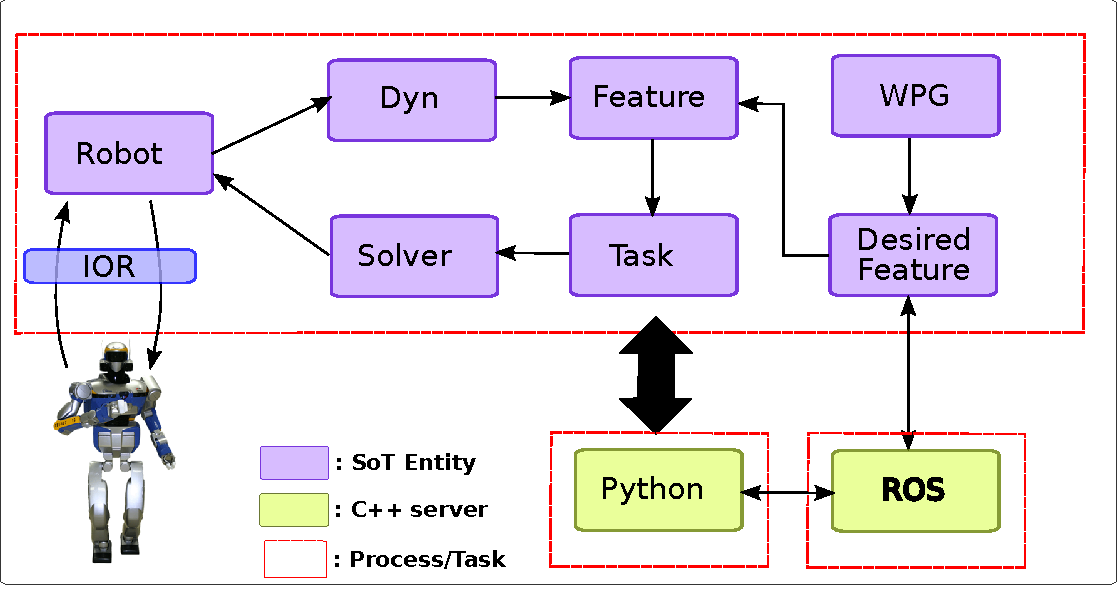
\includegraphics[width=\linewidth]{./figures/Concept-Fig}
  \end{figure}
\end{frame}

\begin{frame}{Software structure - Link with Model}
  \begin{figure}
    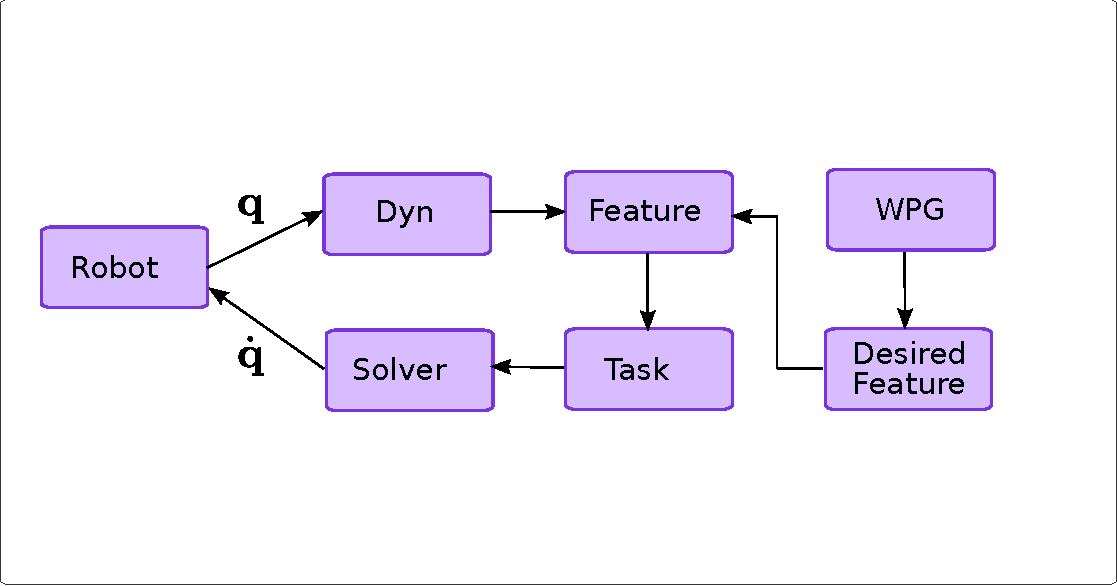
\includegraphics[width=\linewidth]{./figures/Concept-Theory-Fig-Finalv2M5}
  \end{figure}
\end{frame}

%  $$ T ({\bf q}, t) = \left(\begin{array}{cc} {\bf t} (M^{* -1}(t) M ({\bf q})) \\ u_{\theta} (R^{* -1}(t) R ({\bf q})) \end{array}\right) $$
    
% $ J=  \frac{\partial T}{\partial {\bf q}}$
 
% $\dot{T} = - \lambda T

% $\dot{T} = - \lambda T - \frac{\partial T}{\partial t} $

% $\dot{{\bf q}} \triangleq& -J ^{+} (\lambda T + \frac{\partial T}{\partial t} $

\begin{frame}{Software structure - Link with Model}
  \begin{figure}
    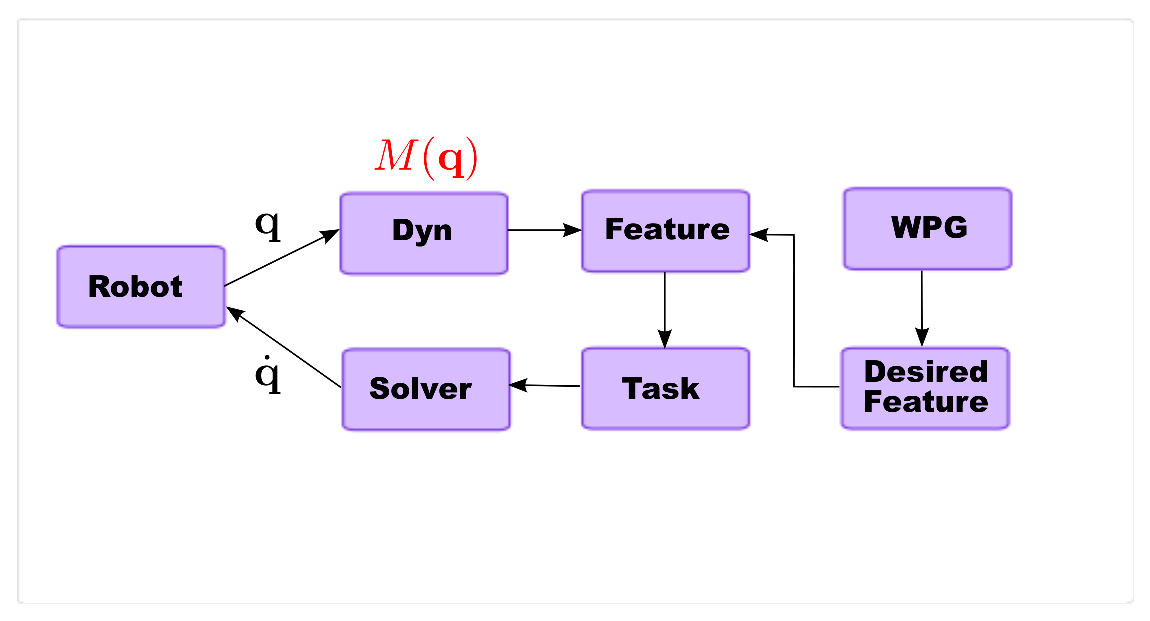
\includegraphics[width=\linewidth]{./figures/Concept-Theory-Fig-Finalv2M4}
  \end{figure}
\end{frame}

\begin{frame}{Software structure - Link with Model}
  \begin{figure}
    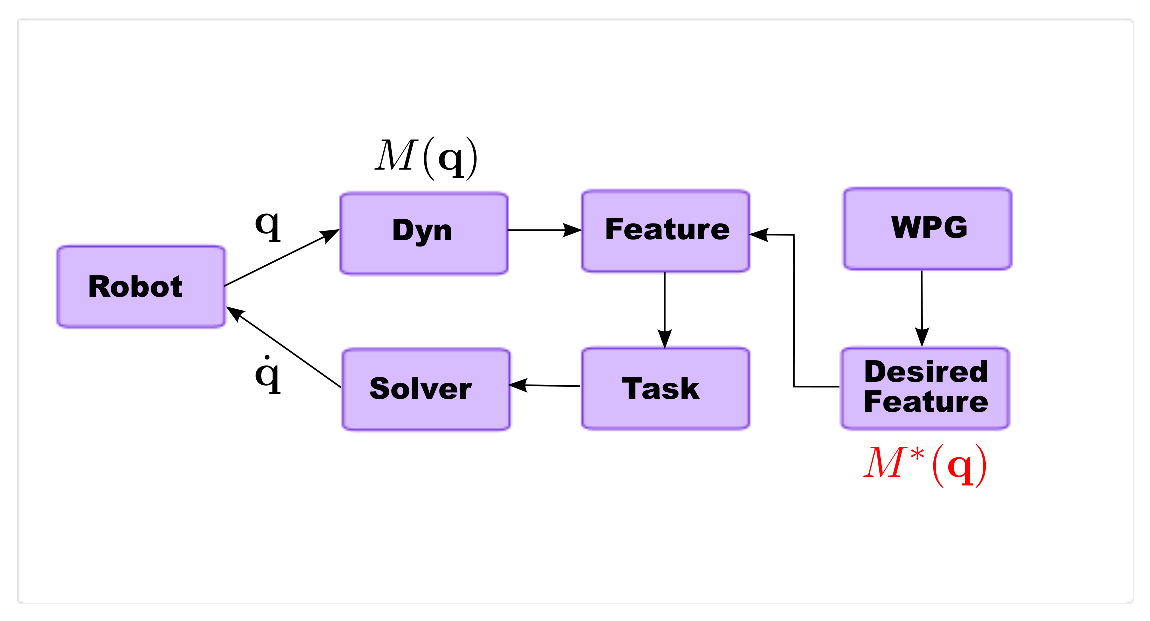
\includegraphics[width=\linewidth]{./figures/Concept-Theory-Fig-Finalv2M3}
  \end{figure}
\end{frame}

\begin{frame}{Software structure - Link with Model}
  \begin{figure}
    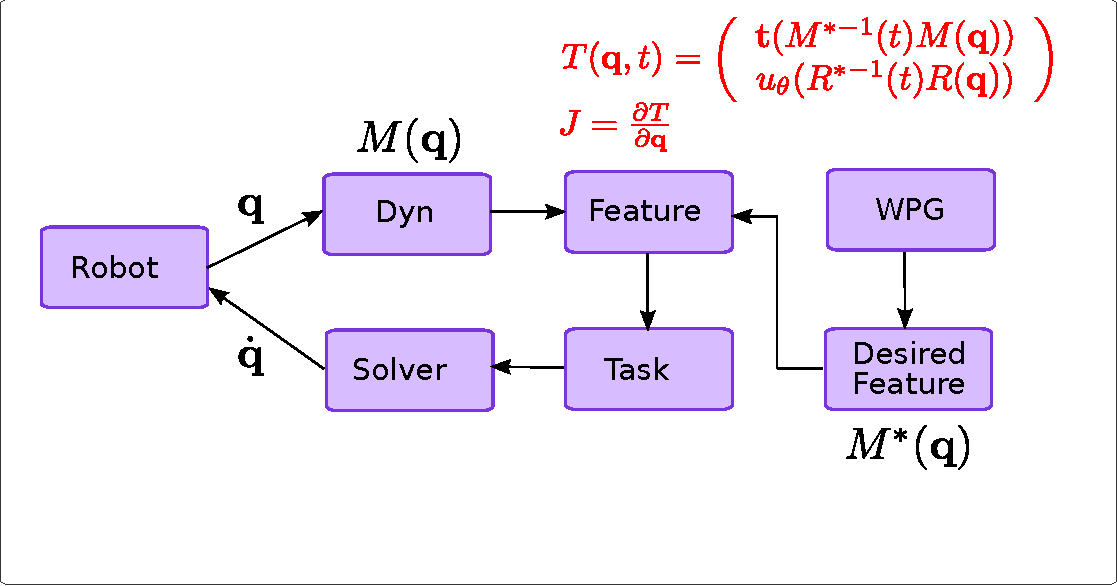
\includegraphics[width=\linewidth]{./figures/Concept-Theory-Fig-Finalv2M2}
  \end{figure}
\end{frame}

\begin{frame}{Software structure - Link with Model}
  \begin{figure}
    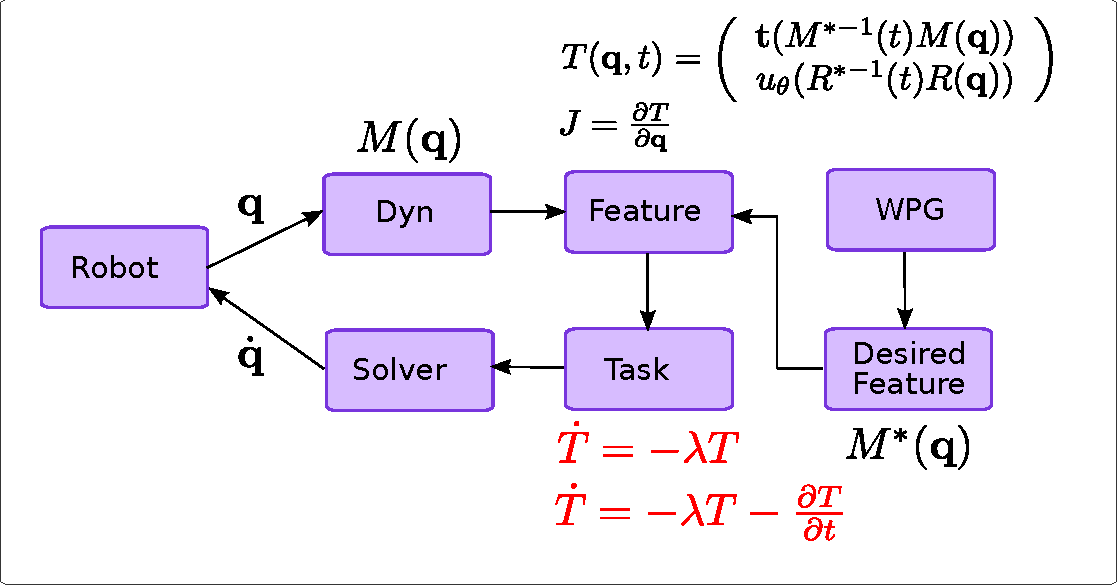
\includegraphics[width=\linewidth]{./figures/Concept-Theory-Fig-Finalv2M1}
  \end{figure}
\end{frame}

\begin{frame}{Software structure - Link with Model}
  \begin{figure}
    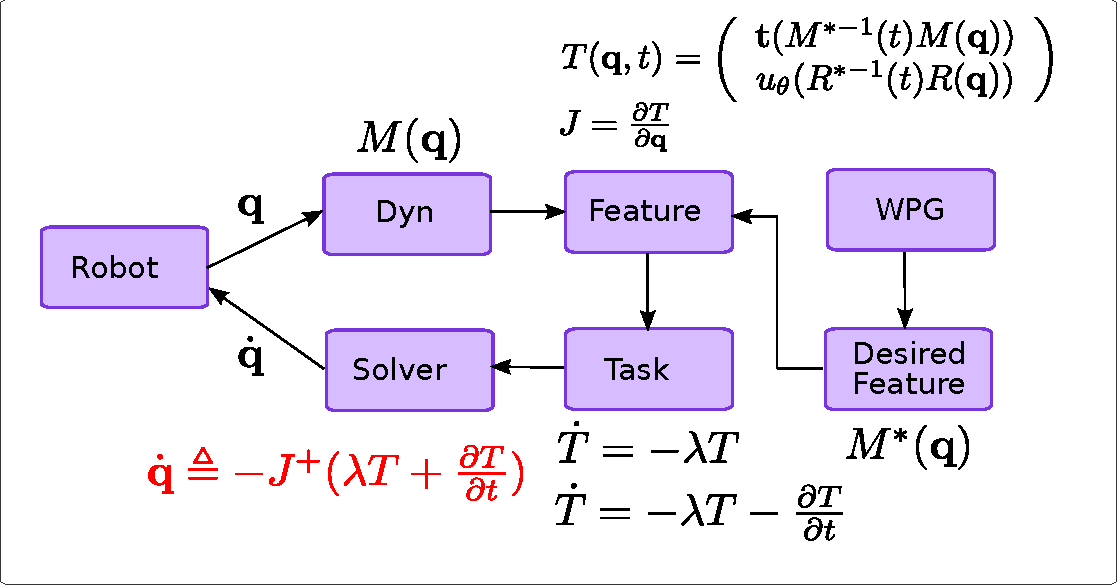
\includegraphics[width=\linewidth]{./figures/Concept-Theory-Fig-Finalv2}
  \end{figure}
\end{frame}

\begin{frame}{Software structure - Repositories}
  \begin{figure}
    \includegraphics[width=\linewidth]{./figures/Concept-Software-Fig}
  \end{figure}
\end{frame}

